% This is part of Mes notes de mathématique
% Copyright (c) 2006-2016
%   Laurent Claessens, Carlotta Donadello
% See the file fdl-1.3.txt for copying conditions.
 
%+++++++++++++++++++++++++++++++++++++++++++++++++++++++++++++++++++++++++++++++++++++++++++++++++++++++++++++++++++++++++++
\section{Suites de fonctions}
%+++++++++++++++++++++++++++++++++++++++++++++++++++++++++++++++++++++++++++++++++++++++++++++++++++++++++++++++++++++++++++

%---------------------------------------------------------------------------------------------------------------------------
\subsection{Convergence de suites de fonctions}
%---------------------------------------------------------------------------------------------------------------------------

Nous considérons un espace normé \( (\Omega,\| . \|)\). Nous disons qu'une suite de fonctions \( f_n\) \defe{converge}{convergence!en norme} vers \( f\) pour la norme \( \| . \|\) si \( \forall \epsilon>0\), \( \exists N\) tel que \( n\geq N\) implique \( \| f_n-f \|<\epsilon\).

Dans le cas particulier de la norme 
\begin{equation}
    \| f \|_{\infty}=\sup_{x\in\Omega}| f(x) |,
\end{equation}
nous parlons que \defe{convergence uniforme}{convergence!uniforme!suite de fonctions}.

\begin{theorem}[Critère de Cauchy]  \label{ThoCauchyZelUF}
    Une suite de fonctions  \( (f_n)_{n\in\eN}\) sur \( \Omega\) converge en norme sur \( \Omega\) si et seulement si \( \forall\epsilon>0\), \( \exists N\) tel que
    \begin{equation}
        \| f_n-f_m \|<\epsilon
    \end{equation}
    pour \( n,m>N\).
\end{theorem}

\begin{corollary}       \label{CorCauchyCkXnvY}
    La série \( \sum f_n\) converge en norme sur \( \Omega\) si et seulement si \( \exists N\) tel que
    \begin{equation}
        \| f_n+\ldots+f_m \|\leq \epsilon
    \end{equation}
    pour tout \( n,m>N\).
\end{corollary}

\begin{proof}
    L'hypothèse montre que la suite des sommes partielles de la série \( \sum f_n\) vérifie le critère de Cauchy du théorème \ref{ThoCauchyZelUF}.
\end{proof}

%--------------------------------------------------------------------------------------------------------------------------- 
\subsection{Convergence uniforme}
%---------------------------------------------------------------------------------------------------------------------------

\begin{definition}[\cite{TrenchRealAnalisys}]
    Nous disons qu'une suite de fonctions \( (f_n)\) définies sur un ensemble \( A\) \defe{converge uniformément}{convergence!uniforme} vers une fonction \( f\) si
    \begin{equation}
        \lim_{n\to \infty} \| f_n-f \|_A=0
    \end{equation}
    où \( \| g \|_A=\sup_{x\in A}\| g(x) \|\).
\end{definition}

\begin{proposition}[Critère de Cauchy uniforme\cite{LCbyNWQ}]   \label{PropNTEynwq}
    Soit \( X\) un espace topologique et \( (Y,d)\) un espace topologique complet. La suite de fonction \( f_n\colon X\to Y\) converge uniformément sur \( A\) si et seulement si pour tout \( \epsilon>0\) il existe \( N\in \eN\) tel que si \( k,l>N\) alors
    \begin{equation}
        d\big( f_k(x),f_l(x) \big)\leq \epsilon
    \end{equation}
    pour tout \( x\in X\).
\end{proposition}
\index{Cauchy!critère!uniforme}
\index{critère!Cauchy!uniforme}
Grosso modo, cela dit que si qu'une suite de Cauchy pour la norme uniforme est une suite uniformément convergente. Le fait que la suite converge fait partie du résultat et n'est pas une hypothèse. Ce critère sera utilisé pour montrer que \( \big( C(K),\| . \|_{\infty} \big)\) est complet, proposition \ref{PropSYMEZGU}. 

\begin{proof}
    Si \( f_n\stackrel{unif}{\longrightarrow}f\) alors le critère est satisfait; c'est dans l'autre sens que la preuve est intéressante.

    Soit donc une suite de fonctions satisfaisant au critère et montrons qu'elle converge uniformément. Pour tout \( x\in X\) la suite \( n\mapsto f_n(x)\) est de Cauchy dans l'espace complet \( Y\); nous avons donc convergence ponctuelle \( f_n\to f\). Nous devons prouver que cette convergence est uniforme. Soit \( \epsilon>0\) et \( N\in \eN\) tel que si \( k,l>N\) alors
    \begin{equation}
        d\big( f_k(x),f_l(x) \big)\leq \epsilon
    \end{equation}
    pour tout \( x\in X\). Si nous nous fixons un tel \( k\) et un \( x\in A\) nous considérons l'inégalité
    \begin{equation}
        d\big( f_k(x),f_l(x) \big)\leq \epsilon
    \end{equation}
    qui est vraie pour tout \( l\). En passant à la limite \( l\to\infty\) (limite qui commute avec la fonction distance par définition de la topologie) nous avons
    \begin{equation}
        d\big( f_k(x),f(x) \big)\leq \epsilon.
    \end{equation}
    Cette inégalité étant valable pour tout \( x\in X\), cela signifie que \( f_n\stackrel{unif}{\longrightarrow}f\).
\end{proof}

\begin{theorem}[Limite uniforme de fonctions continues]			\label{ThoUnigCvCont}
    Soit \( A\), un ensemble mesuré et \( f_n\colon A\to \eR^n\), une suite de fonctions continues convergeant uniformément vers \( f\). Si les fonctions \( f_n\) sont toutes continues en \( x_0\in A\), alors \( f\) est continue en \( x_0\).
\end{theorem}

\begin{proof}
    Soit \( \epsilon>0\). Si \( x\in A\) nous avons, pour tout \( n\), la majoration
    \begin{subequations}
        \begin{align}
            \| f(x)-f(x_0) \|&\leq \| f(x)-f_n(x) \|+\| f_n(x)-f_n(x_0) \|+\| f_n(x_0)-f(x_0) \|\\
            &\leq\| f_n(x)-f_n(x_0) \|+2\| f_n-f \|_{\infty}.
        \end{align}
    \end{subequations}
    Grâce à l'uniforme convergence, nous considérons \(N\in \eN\) tel que \( \| f_n-f \|\leq \epsilon\) pour tout \( n\geq N\). Pour de tels \( n\), nous avons
    \begin{equation}
        \| f(x)-f(x_0) \|\leq 2\epsilon\| f_n-f \|+\| f_n(x)-f_n(x_0) \|.
    \end{equation}
    La continuité de \( f_n\) nous fournit un \( \delta>0\) tel que \( \| f_n(x_0)-f_n(x) \|<\epsilon\) dès que \( \| x-x_0 \|<\delta\). Pour ce \( \delta\), nous avons alors \( \| f(x)-f(x_0) \|<\epsilon\).
\end{proof}

\begin{theorem}[Théorème de Dini\cite{JIFGuct}] \label{ThoUFPLEZh}
    Soit \( D\) un espace métrique compact et une suite de fonctions \( f_n\in C(D,\eR)\) telle que
    \begin{enumerate}
        \item
            \( f_n\to g\) ponctuellement,
        \item
            \( g\in C(D,\eR)\),
        \item
            la suite \( (f_n)\) est croissante, c'est à dire que pour tout \( x\in D\) et pour tout \( n\geq 0\) nous avons \( f_{n+1}(x)\geq f_n(x)\).
    \end{enumerate}
    Alors la convergence est uniforme.
\end{theorem}
\index{convergence!uniforme!théorème de Dini}
\index{compacité!théorème de Dini}
\index{théorème!Dini}

\begin{proof}
    Soit \( x\in D\) et \( \epsilon>0\). Il existe \( N(x)\in \eN\) tel que
    \begin{equation}
        g(x)-\epsilon\leq f_{N(x)}\leq g(x).
    \end{equation}
    De plus \( g\) et \( f_{N(x)}\) sont des fonctions continues, donc il existe \( \eta(x)\) tel que si \( y\in B\big( x,\eta(x) \big)\) alors
    \begin{subequations}
        \begin{align}
            g(y)&\in B\big( g(x),\epsilon \big) \label{subEqXKjgKgv}\\
            f_{N(x)}(y)&\in B\big( f_{N(x)}(x),\epsilon \big)   \label{subEqHTiYZLd}.
        \end{align}
    \end{subequations}
    Si \( n\geq N(x)\) et si \( y\in B(x,\eta(x))\) alors nous avons les majorations
    \begin{equation}
            g(y)\geq f_n(y)
            \geq f_{N(x)}(y)
            \geq f_{N(x)}(x)-\epsilon
            \geq g(x)-2\epsilon
            \geq g(y)-3\epsilon.
    \end{equation}
    Justifications :
    \begin{multicols}{2}
        \begin{enumerate}
            \item
                Les deux première inégalités sont la croissance de la suite.
            \item
                La suivante est \eqref{subEqHTiYZLd}.
            \item
                Ensuite il y a le choix de \( N(x)\).
            \item
                Et enfin il y a \eqref{subEqXKjgKgv}.
        \end{enumerate}
    \end{multicols}
    Nous retenons que si \( x\in D\) et si \( n\geq N(x)\) alors
    \begin{equation}    \label{EqJCMktdj}
        g(y)\geq f_n(y)\geq g(y)-3\epsilon
    \end{equation}
    pour tout \( y\in B(x,\eta(x))\).

    Nous utilisons maintenant la compacité de \( D\). Pour chaque \( x\in D\) nous pouvons considérer la boule ouverte \( B\big( x,\eta(x) \big)\); ces boules recouvrent \( D\). Nous en extrayons un sous-recouvrement fini, c'est à dire un ensemble fini d'éléments \( x_1\),\ldots, \( x_K\) tels que
    \begin{equation}
        D=\bigcup_{k=1}^K B\big(x_k,\eta(x_k)\big).
    \end{equation}
    Si à ce moment vous ne comprenez pas pourquoi c'est une égalité au lieu d'une inclusion, il faut lire l'exemple \ref{ExKYZwYxn}. Considérons 
    \begin{equation}
        n\geq N=\max\{ N(x_1),\ldots, N(x_K) \}.
    \end{equation}
    Pour tout \( y\in D\) il existe \( k\in\{ 1,\ldots, K \}\) tel que \( y\in B\big( x_k,\eta(x_k) \big)\), et vu que \( n\geq N(x_k)\) nous reprenons la majoration \eqref{EqJCMktdj} :
    \begin{equation}
        g(y)\geq f_n(y)\geq g(y)-3\epsilon.
    \end{equation}
    Pour le \( n\) choisi nous avons ces inégalités pour tout \( y\in D\), c'est à dire que nous avons \( \| f_n-g \|\leq 3\epsilon\) et donc la convergence uniforme.
\end{proof}

%--------------------------------------------------------------------------------------------------------------------------- 
\subsection{Permuter avec les dérivées partielles}
%---------------------------------------------------------------------------------------------------------------------------

\begin{theorem}		\label{ThoSerUnifDerr}
	Soit $U\subset\eR^n$ ouvert, $f_k\colon U\to \eR$ et $f_k$ de classe $C^1$. Supposons que $f_k$ converge simplement vers $f$ et que $\partial_if_k$ converge uniformément sur tout compact  vers une fonction $g_i$ pour $i=1,\ldots,n$. Alors $f$ est de classe $C^1$ et $\partial_if=g_i$. De plus, $f_k$ converge vers $f$ uniformément.
\end{theorem}
\index{permuter!dérivée et limite}
%TODO : une preuve.


%+++++++++++++++++++++++++++++++++++++++++++++++++++++++++++++++++++++++++++++++++++++++++++++++++++++++++++++++++++++++++++
\section{Recherche d'extrema}
%+++++++++++++++++++++++++++++++++++++++++++++++++++++++++++++++++++++++++++++++++++++++++++++++++++++++++++++++++++++++++++

Soit une fonction $f\colon I\to \eR$, et soit $a\in I$. Si $f'(a)>0$, alors la tangente au graphe de $f$ au point $\big( a,f(a) \big)$ sera une droite croissante (coefficient directeur positif). Cela ne veut pas spécialement dire que la fonction elle-même sera croissante, mais en tout cas cela est un bon indice.

\begin{example}
	Si $f(x)=x^2$, il est connu que $f'(x)=2x$. Nous avons donc que $f'$ est positive si $x\geq 0$ et $f'>$ est négative si $x<0$. Cela correspond bien au fait que $x^2$ est décroissante sur $\mathopen] -\infty , 0 \mathclose[$ et croissante sur $\mathopen] 0 , \infty \mathclose[$.
\end{example}
 
Sur la figure \ref{LabelFigWIRAooTCcpOV}, nous avons dessiné la fonction $f(x)=x\cos(x)$ et sa dérivée. Nous voyons que partout où la dérivée est négative, la fonction est décroissante tandis que, inversement, partout où la dérivée est positive, la fonction est croissante.
\newcommand{\CaptionFigWIRAooTCcpOV}{La fonction $f(x)=x\cos(x)$ en bleu et sa dérivée en rouge.}
\input{Fig_WIRAooTCcpOV.pstricks}

Les extrema de la fonction $f$ sont donc placés là où $f'$ change de signe. En effet si $f'(x)<0$ pour $x<a$ et $f'(x)>0$ pour $x>a$, la fonction est décroissante jusqu'à $a$ et est ensuite croissante. Cela signifie que la fonction connait un creux en $a$. Le point $a$ est donc un minimum de la fonction.

Attention cependant. Le fait que $f'(a)=0$ ne signifie pas automatiquement que $f$ a un maximum ou un minimum en $a$. Nous avons par exemple tracé sur la figure \ref{LabelFigVBOIooRHhKOH} les fonctions $x^3$ et sa dérivée. Il est à noter que, conformément à ce que l'on pense, certes la dérivée s'annule en $x=0$, mais elle ne change pas de signe.

\newcommand{\CaptionFigVBOIooRHhKOH}{La dérivée de $x^3$ s'annule en $x=0$, mais ce n'est ni un minimum ni un maximum.}
\input{Fig_VBOIooRHhKOH.pstricks}


%+++++++++++++++++++++++++++++++++++++++++++++++++++++++++++++++++++++++++++++++++++++++++++++++++++++++++++++++++++++++++++ 
\section{Fonctions réelles de deux variables réelles}
%+++++++++++++++++++++++++++++++++++++++++++++++++++++++++++++++++++++++++++++++++++++++++++++++++++++++++++++++++++++++++++

Une \textbf{fonction réelle de 2 variables réelles} est une fonction $f : A \subset \eR^2 \to \eR : (x,y) \mapsto z = f(x,y)$.

Le \textbf{graphe de $f$}, noté $\Graphe f$, est un sous-ensemble de $\eR^3$:\[\Graphe f = \{(x,y,z) \in \eR^3 \mid (x,y) \in A \text{ et } z = f(x,y)\}\]

Les \textbf{courbes de niveau} de la fonction $f$ sont obtenues en posant $f(x,y)=\lambda$.

%---------------------------------------------------------------------------------------------------------------------------
\subsection{Limites de fonctions à deux variables}
%---------------------------------------------------------------------------------------------------------------------------

Ici nous n'allons pas entrer dans tous les détails, mais simplement mentionner les quelques techniques les plus courantes. 

\begin{theorem}		\label{ThoLimiteCompose}
	Soient deux fonctions $f\colon \eR^n\to \eR^p$ et $g\colon \eR^p\to \eR^q$. Si $a$ est un point adhérent au domaine de $g\circ f$ et si
	\begin{equation}
		\begin{aligned}[]
			\lim_{x\to a}f(x)&=b\\
			\lim_{y\to b}g(y)&=c,
		\end{aligned}
	\end{equation}
	alors 
	\begin{equation}
		\lim_{x\to a}(g\circ f)(x)=c.
	\end{equation}
\end{theorem}

Les techniques usuelles sont
\begin{enumerate}

	\item
		La règle de l'étau. Cette technique demande un peu plus d'imagination parce qu'il faut penser à un «truc» différent pour chaque exercice. En revanche, la justification est facile : il y a un théorème qui dit que ça marche.

	\item
		Lorsqu'on applique la règle de l'étau, penser à
		\begin{equation}
			| x |=\sqrt{x^2}\leq\sqrt{x^2+y^2}.
		\end{equation}
		Cela permet de majorer le numérateur. Attention : ce genre de majoration ne fonctionnent qu'au numérateur : agrandir le dénominateur ferait diminuer la fraction.

	\item
		Il n'est pas vrai que
		\begin{equation}
			| x |=\sqrt{x^2}\leq\sqrt{x^4}\leq\sqrt{x^4+2y^4}.
		\end{equation}
		En effet, si $x$ est petit, alors $x^2>x^4$, et non le contraire.

\end{enumerate}

Une technique très efficace pour les limites $(x,y)\to (0,0)$ est le passage aux coordonnées polaires. Il s'agit de poser
\begin{subequations}
	\begin{numcases}{}
		x=r\cos(\theta)\\
		y=r\sin(\theta)
	\end{numcases}
\end{subequations}
et puis de faire la limite $r\to 0$.

Si la limite obtenue {\bf ne dépend pas de $\theta$}, alors c'est la limite cherchée. L'exercice suivant en donne des exemples.
\Exo{mazhe-0000}

%---------------------------------------------------------------------------------------------------------------------------
\subsection{Dérivées partielles}
%---------------------------------------------------------------------------------------------------------------------------

La \defe{dérivée partielle}{dérivée!partielle} par rapport à $x$ au point $(x,y)$ est notée
\begin{equation}
	\frac{\partial f}{\partial x}(x,y) 
\end{equation}
et se calcule en dérivant $f$ par rapport  à $x$ en considérant que $y$ est constante.

De la même manière, la dérivée partielle par rapport à $y$ au point $(x,y)$ est notée
\begin{equation}
	\frac{\partial f}{\partial y}(x,y) 
\end{equation}
et se calcule en dérivant $f$ par rapport  à $y$ en considérant que $x$ est constante.

Pour les dérivées partielles secondes,
\begin{itemize}
\item $f''_{xx} (x,y) = (f'_x)'_x = \frac{\partial^2 f}{\partial x^2}(x,y) = \frac{\partial}{\partial x}(\frac{\partial f}{\partial x})$.
\item $f''_{yy} (x,y) = (f'_y)'_y = \frac{\partial^2 f}{\partial y^2}(x,y) = \frac{\partial}{\partial y}(\frac{\partial f}{\partial y})$.
\item $f''_{xy} (x,y) = (f'_x)'_y  = (f'_y)'_x = f''_{yx} (x,y) \text{ ou } \frac{\partial^2 f}{\partial x \partial y}(x,y) = \frac{\partial}{\partial x}(\frac{\partial f}{\partial y})  = \frac{\partial}{\partial y}(\frac{\partial f}{\partial x}) =\frac{\partial^2 f}{\partial y \partial x}(x,y)$.
\end{itemize}

%---------------------------------------------------------------------------------------------------------------------------
\subsection{Différentielle et accroissement}
%---------------------------------------------------------------------------------------------------------------------------

La \defe{différentielle totale}{différentielle!totale} de $f$ au point $(a,b)$ est donnée, quand elle existe (!), par la formule
\begin{equation}
	df(a,b) = \frac{\partial f}{\partial x}(a,b)dx + \frac{\partial f}{\partial y}(a,b) dy.
\end{equation}

De la même façon que la formule des accroissements finis disait que $f(x+a)\simeq f(x)+af'(x)$, en deux dimensions nous avons que l'\defe{accroissement}{accroissement} approximatif de $f$ au point $(a,b)$ pour des accroissements $\Delta x$ et $\Delta y$ est 
\begin{equation}
	f(x+\Delta x,y+\Delta y)=f(x,y)+\Delta x\frac{ \partial f }{ \partial x }(x,y)+\Delta y\frac{ \partial f }{ \partial y }(x,y).
\end{equation}

%TODO : pour l'index, l'expression régulière suivante aide :
% grep "defe{[A-Za-z ]*}{[A-Z]" *.tex
Le \defe{plan tangent}{plan!tangent} au graphe de $f$ au point $\big(a,b,f(a,b)\big)$ est 
\begin{equation}
	T_{(a,b)}(x,y) = f(a,b) + \frac{\partial f}{\partial x}(a,b) (x-a) + \frac{\partial f}{\partial y}(a,b) (y-b)
\end{equation}
essayez d'écrire l'équation de la droite tangente au graphe de $f(x)$ au point $x=a$ en terme de la dérivée de $f$, et comparez votre résultat à cette formule.

Un des principaux théorèmes pour tester la différentiabilité d'une fonction est le suivant.

\begin{theorem}		\label{ThoProuverDiffable}
	Soit une fonction $f\colon \eR^m\to \eR^p$. Si les dérivées partielles existent dans un voisinage de $a$ et donc continues en $a$, alors $f$ est différentiable en $a$.
\end{theorem}
Le plus souvent, nous prouvons qu'une fonction est différentiable en calculant les dérivées partielles et en montrant qu'elles sont continues.

%---------------------------------------------------------------------------------------------------------------------------
\subsection{Recherche d'extrema locaux}
%---------------------------------------------------------------------------------------------------------------------------

\begin{enumerate}
\item Rechercher les points critiques, càd les $(x,y)$ tels que
\[\begin{cases} \frac{\partial f}{\partial x}(x,y) = 0 \\ \frac{\partial f}{\partial y}(x,y) = 0 \end{cases} \]
En effet, si $(x_0,y_0)$ est un extrémum local de $f$, alors $\frac{\partial f}{\partial x}(x_0,y_0) = 0 = \frac{\partial f}{\partial y}(x_0,y_0)$.
\item Déterminer la nature des points critiques: «test» des dérivées secondes:
\[\text{On pose }H(x_0,y_0) = \frac{\partial^2 f}{\partial x^2}(x_0,y_0)\frac{\partial f^2}{\partial y^2}(x_0,y_0) - \left(\frac{\partial^2 f}{\partial x\partial y}(x_0,y_0)\right)^2\]
\begin{enumerate}
\item Si $H(x_0,y_0) > 0$ et $\frac{\partial^2 f}{\partial x^2}(x_0,y_0) > 0 \Longrightarrow (x_0,y_0)$ est un minimum local de $f$.
\item Si $H(x_0,y_0) > 0$ et $\frac{\partial^2 f}{\partial x^2}(x_0,y_0) < 0 \Longrightarrow (x_0,y_0)$ est un maximum local de $f$.
\item Si $H(x_0,y_0) < 0 \Longrightarrow f$ a un point de selle en $(x_0,y_0)$.
\item Si $H(x_0,y_0) = 0 \Longrightarrow$ on ne peut rien conclure.
\end{enumerate}
\end{enumerate}

\textbf{Dérivation implicite:} Soit $F(x,f(x)) = 0$ la représentation implicite d'une fonction $y=f(x)$ alors \[y' = f'(x) = - \frac{F'_x}{F'_y}.\]


%+++++++++++++++++++++++++++++++++++++++++++++++++++++++++++++++++++++++++++++++++++++++++++++++++++++++++++++++++++++++++++
\section{Les fonctions à valeurs vectorielles}
%+++++++++++++++++++++++++++++++++++++++++++++++++++++++++++++++++++++++++++++++++++++++++++++++++++++++++++++++++++++++++++

Jusqu'à présent nous avons vu des fonctions de plusieurs variables qui prenaient leurs valeurs dans $\eR$. Nous allons maintenant voir ce qu'il se passe lorsque les fonctions prennent leurs valeurs dans $\eR^3$.

Une fonction d'une variable est dite \defe{à valeurs vectorielles}{fonction!valeurs vectorielles} lorsque
\begin{equation}
    \begin{aligned}
        f\colon I\subset \eR&\to \eR^3 \\
        f(x)&=\begin{pmatrix}
            f_1(x)    \\ 
            f_2(x)    \\ 
            f_3(x)    
        \end{pmatrix}.
    \end{aligned}
\end{equation}
Les fonctions $f_i\colon \eR\to \eR$ sont les \defe{composantes}{composante} de $f$. Ce que nous avons raconté à propos des dérivées passe facilement :
\begin{equation}
    \frac{ f(a+\epsilon)-f(a) }{ \epsilon }=
    \begin{pmatrix}
        \frac{ f_1(a+\epsilon)-f_1(a) }{ \epsilon }    \\ 
        \frac{ f_2(a+\epsilon)-f_2(a) }{ \epsilon }    \\ 
        \frac{ f_3(a+\epsilon)-f_3(a) }{ \epsilon }    
    \end{pmatrix}.
\end{equation}
En particulier dès que les fonctions $f_i$ sont dérivables, nous avons
\begin{equation}
    f'(a)=\begin{pmatrix}
        f_1'(a)    \\ 
        f_2'(a)    \\ 
        f_3'(a)    
    \end{pmatrix}
\end{equation}
comme dérivée de la fonction. Cette dérivée est un vecteur.

\begin{example}
    Si
    \begin{equation}
        f\colon x\in\eR\mapsto \begin{pmatrix}
            x^2 e^{x}    \\ 
            \cos(x^2)    \\ 
            x^3+x    
        \end{pmatrix},
    \end{equation}
    alors
    \begin{equation}
        f'(x)=\begin{pmatrix}
            2xe^x+x^2e^x    \\ 
            -2x\sin(x^2)    \\ 
            3x^2+1    
        \end{pmatrix}.
    \end{equation}
\end{example}

%+++++++++++++++++++++++++++++++++++++++++++++++++++++++++++++++++++++++++++++++++++++++++++++++++++++++++++++++++++++++++++
\section{Fonctions vectorielles de plusieurs variables}
%+++++++++++++++++++++++++++++++++++++++++++++++++++++++++++++++++++++++++++++++++++++++++++++++++++++++++++++++++++++++++++

Ce sont les fonctions de la forme
\begin{equation}
    \begin{aligned}
        f\colon \eR^3&\to \eR^3 \\
        \begin{pmatrix}
            x    \\ 
            y    \\ 
            z    
        \end{pmatrix}&\mapsto \begin{pmatrix}
            f_1(x,y,z)\\
            f_2(x,y,z)\\
            f_3(x,y,z)
        \end{pmatrix}.
    \end{aligned}
\end{equation}

En ce qui concerne les dérivées, tout se passe comme avant. Si les dérivées partielles des composantes $f_i$ existent au point $a\in\eR^3$, alors
\begin{equation}
    \begin{aligned}[]
        \frac{ \partial f }{ \partial x }(a)&=\begin{pmatrix}
            \partial_xf_1(a)    \\ 
            \partial_xf_2(a)    \\ 
            \partial_xf_3(a)    \\ 
        \end{pmatrix},&
        \frac{ \partial f }{ \partial y }(a)&=\begin{pmatrix}
            \partial_yf_1(a)    \\ 
            \partial_yf_2(a)    \\ 
            \partial_yf_3(a)    \\ 
        \end{pmatrix},&
        \frac{ \partial f }{ \partial z }(a)&=\begin{pmatrix}
            \partial_zf_1(a)    \\ 
            \partial_zf_2(a)    \\ 
            \partial_zf_3(a)    \\ 
        \end{pmatrix}.
    \end{aligned}
\end{equation}

%+++++++++++++++++++++++++++++++++++++++++++++++++++++++++++++++++++++++++++++++++++++++++++++++++++++++++++++++++++++++++++
\section{Champs de vecteurs}
%+++++++++++++++++++++++++++++++++++++++++++++++++++++++++++++++++++++++++++++++++++++++++++++++++++++++++++++++++++++++++++

Un champ de vecteur est une fonction $f\colon \eR^3\to \eR^3$. Géométriquement, il s'agit simplement de mettre un vecteur en chaque point de l'espace. Cela arrive très souvent en physique.

\begin{example}
    Si un fluide (eau, gaz) coule dans un tube, en tout point le point a une vitesse, qui sera un vecteur généralement dirigé le long du tube.
\end{example}

\begin{example}
    La force d'attraction de la Terre sur une masse $m$ située au point $r=(x,y,z)$ est donnée par
    \begin{equation}
        F(r)=-G\frac{ Mmr }{ \| r \|^3 }.
    \end{equation}
    Dans cette expression, tant $r$ que $F(r)$ sont des vecteurs. Nous l'avons représenté sur la figure \ref{LabelFigSQNPooPTrLRQ}. % From file SQNPooPTrLRQ
\newcommand{\CaptionFigSQNPooPTrLRQ}{Le champ de gravitation de la Terre.}
\input{Fig_SQNPooPTrLRQ.pstricks}

    L'application
    \begin{equation}
        \begin{aligned}
            F\colon \eR^3&\to \eR^3 \\
            r&\mapsto F(r) 
        \end{aligned}
    \end{equation}
    est le champ gravitationnel de la Terre.

\end{example}

%---------------------------------------------------------------------------------------------------------------------------
\subsection{Matrice jacobienne}
%---------------------------------------------------------------------------------------------------------------------------

La \defe{matrice jacobienne}{jacobien} de la fonction $f\colon \eR^3\to \eR^3$ au point $a\in\eR^3$ est la matrice dont les colonnes sont les vecteurs $\frac{ \partial f }{ \partial x }(a)$, $\frac{ \partial f }{ \partial y }(a)$ et $\frac{ \partial f }{ \partial z }(a)$, c'est à dire
\begin{equation}
    J_f(a)=\begin{pmatrix}
        \frac{ \partial f_1 }{ \partial x }(a)   &   \frac{ \partial f_1 }{ \partial y }(a)    &   \frac{ \partial f_1 }{ \partial z }(a)    \\
        \frac{ \partial f_2 }{ \partial x }(a)   &   \frac{ \partial f_2 }{ \partial y }(a)    &   \frac{ \partial f_2 }{ \partial z }(a)    \\
        \frac{ \partial f_3 }{ \partial x }(a)   &   \frac{ \partial f_3 }{ \partial y }(a)    &   \frac{ \partial f_3 }{ \partial z }(a)    
    \end{pmatrix}.
\end{equation}

\begin{example}
    Si 
    \begin{equation}
        f(x,y,z)=\begin{pmatrix}
            xy e^{z}    \\ 
            x^2+\cos(yz)    \\ 
            xyz    
        \end{pmatrix},
    \end{equation}
    alors
    \begin{equation}
        J_f(x,y,z)=\begin{pmatrix}
            ye^z    &   xe^z    &   xye^z    \\
            2x    &   -z\sin(yz)    &   -y\sin(yz)    \\
            yz    &   xz    &   xy
        \end{pmatrix}.
    \end{equation}
\end{example}

%+++++++++++++++++++++++++++++++++++++++++++++++++++++++++++++++++++++++++++++++++++++++++++++++++++++++++++++++++++++++++++
\section{Divergence, rotationnel et l'opérateur nabla}
%+++++++++++++++++++++++++++++++++++++++++++++++++++++++++++++++++++++++++++++++++++++++++++++++++++++++++++++++++++++++++++

Nous avons déjà vu le gradient d'une fonction $f\colon \eR^3\to \eR$
\begin{equation}        \label{EqDefNablaf}
    \nabla f(x,y,z)=\begin{pmatrix}
        \partial_xf(x,y,z)    \\ 
        \partial_yf(x,y,z)    \\ 
        \partial_zf(x,y,z)    
    \end{pmatrix}
\end{equation}
Afin de définir la divergence et le rotationnel, nous introduisons $\nabla$ sous une forme un peu plus abstraite comme le «vecteur»
\begin{equation}
    \nabla=\begin{pmatrix}
        \partial_x    \\ 
        \partial_y    \\ 
        \partial_z
    \end{pmatrix}.
\end{equation}
Vue comme ça, la formule \eqref{EqDefNablaf} est claire.

Si $F$ est un champ de vecteurs, nous introduisons la \defe{divergence}{divergence} de $F$ par
\begin{equation}
    \nabla\cdot F=\frac{ \partial F_x }{ \partial x }+\frac{ \partial F_y }{ \partial y }+\frac{ \partial F_z }{ \partial z }.
\end{equation}
Cela est une fonction. Et nous introduisons le rotationnel du champ de vecteur $F$ par
\begin{equation}
    \begin{aligned}[]
        \nabla\times F&=\begin{vmatrix}
              e_x  &   e_y    &   e_z    \\
            \partial_x    &   \partial_y    &   \partial_z    \\
            F_x    &   F_y    &   F_z
        \end{vmatrix}\\
        &=
        \left( \frac{ \partial F_z }{ \partial y }-\frac{ \partial F_y }{ \partial z } \right)e_x
        -\left( \frac{ \partial F_z }{ \partial x }-\frac{ \partial F_x }{ \partial z } \right)e_y
        +\left( \frac{ \partial F_y }{ \partial x }-\frac{ \partial F_x }{ \partial y } \right)e_z.
    \end{aligned}
\end{equation}
Cela est un champ de vecteur. En utilisant le symbole complètement antisymétrique \( \epsilon_{ijk}\), le rotationnel d'un champ de vecteur peut s'écrire
\begin{equation}
    \nabla\times F=\sum_{ijk}\epsilon_{ijk}\partial_i F_j e_k.
\end{equation}

Le gradient, la divergence et le rotationnel consistent à appliquer simplement à $\nabla$ est trois produits qu'on peut effectuer sur un vecteur:
\begin{enumerate}
    \item
        Le produit d'un vecteur par un scalaire multiplie chacune des composantes :
        \begin{equation}
            \begin{pmatrix}
                \partial_x    \\ 
                \partial_y    \\ 
                \partial_z    
            \end{pmatrix}f
            =\begin{pmatrix}
                \partial_xf    \\ 
                \partial_yf    \\ 
                \partial_zf    
            \end{pmatrix}.
        \end{equation}
    \item
        Le produit scalaire d'un vecteur avec un autre vecteur donne lieu à la divergence :
        \begin{equation}
            \begin{pmatrix}
                \partial_x    \\ 
                \partial_y    \\ 
                \partial_z    
            \end{pmatrix}\cdot
            \begin{pmatrix}
                F_x    \\ 
                F_y    \\ 
                F_z    
            \end{pmatrix}=
            \frac{ \partial F_x }{ \partial x }+\frac{ \partial F_y }{ \partial y }+\frac{ \partial F_z }{ \partial z }.
        \end{equation}
    \item
        Le produit vectoriel de deux vecteurs :
        \begin{equation}
            \begin{pmatrix}
                \partial_x    \\ 
                \partial_y    \\ 
                \partial_z    
            \end{pmatrix}\times\begin{pmatrix}
                F_x    \\ 
                F_y    \\ 
                F_z    
            \end{pmatrix}=
            \begin{vmatrix}
                e_x    &   e_y    &   e_z    \\
                \partial_x    &   \partial_y    &   \partial_z    \\
                F_x    &   F_y    &   F_z
            \end{vmatrix}.
        \end{equation}
\end{enumerate}
Ces trois opérations joueront un rôle central en électromagnétisme dans les équations de Maxwell.

\begin{example}
    Soit $F(x,y,z)=x e_x+xy e_y+e_z$, c'est à dire
    \begin{equation}
        F(x,y,z)=\begin{pmatrix}
            x    \\ 
            xy    \\ 
            1    
        \end{pmatrix}.
    \end{equation}
    Son rotationnel est donné par
    \begin{equation}
        \nabla\times F=\begin{vmatrix}
            e_x    &   e_y    &   e_z    \\
            \frac{ \partial  }{ \partial x }    &   \frac{ \partial  }{ \partial y }    &   \frac{ \partial  }{ \partial y }    \\
            x    &   xy    &   1
        \end{vmatrix}=
        (0-0)e_x-(0-0)e_y+(y-0)e_z=ye_z=\begin{pmatrix}
            0    \\ 
            0    \\ 
            y    
        \end{pmatrix}.
    \end{equation}
\end{example}

Afin d'étudier comment se comporte la composition de ces opérateurs, nous aurons besoin de ce lemme que nous n'énoncerons pas précisément.
\begin{lemma}       \label{LemPermDerrxyz}
    Si $f\colon \eR^3\to \eR$ est une fonction de classe $C^2$, alors on peut permuter l'ordre des dérivées:
    \begin{equation}
        \begin{aligned}[]
            \frac{ \partial  }{ \partial x }\left( \frac{ \partial f }{ \partial y } \right)&=\frac{ \partial  }{ \partial y }\left( \frac{ \partial f }{ \partial x } \right)\\
            \frac{ \partial  }{ \partial x }\left( \frac{ \partial f }{ \partial z } \right)&=\frac{ \partial  }{ \partial z }\left( \frac{ \partial f }{ \partial x } \right)\\
            \frac{ \partial  }{ \partial z }\left( \frac{ \partial f }{ \partial y } \right)&=\frac{ \partial  }{ \partial y }\left( \frac{ \partial f }{ \partial z } \right)
        \end{aligned}
    \end{equation}
\end{lemma}
La fonction
\begin{equation}
    (x,y,z)\mapsto\frac{ \partial  }{ \partial x }\left( \frac{ \partial f }{ \partial y } \right)(x,y,z)
\end{equation}
sera notée
\begin{equation}
    \frac{ \partial^2f }{ \partial x\partial y }.
\end{equation}

Il y a deux propriétés importantes :
\begin{theorem}
    Soit $f\colon \eR^3\to \eR$ une fonction de classe $C^2$. Alors
    \begin{equation}
        \nabla\times(\nabla f)=0.
    \end{equation}
    Si $F\colon \eR^3\to \eR^3$ est un champ de vecteurs de classe $C^2$, alors
    \begin{equation}
        \nabla\cdot(\nabla\times F)=0.
    \end{equation}
\end{theorem}

\begin{proof}
    Ce sont seulement deux calculs qui manipulent les définitions. Pour le premier, la divergence de $f$ est le champ de vecteurs
    \begin{equation}
        \nabla f=\frac{ \partial f }{ \partial x }e_x+\frac{ \partial f }{ \partial y }e_y+\frac{ \partial f }{ \partial z }e_z.
    \end{equation}
    En mettant ce champ dans la définition du rotationnel,
    \begin{equation}
        \begin{aligned}[]
            \nabla\times(\nabla f)=\begin{vmatrix}
                 e_x   &   e_y    &   e_z    \\
                 \frac{ \partial  }{ \partial x }    &   \frac{ \partial  }{ \partial y }    &   \frac{ \partial  }{ \partial z }    \\
                 \frac{ \partial f }{ \partial x }    &   \frac{ \partial f }{ \partial y }    &   \frac{ \partial f }{ \partial z }
            \end{vmatrix}
            &=\left[ \frac{ \partial  }{ \partial y }\left( \frac{ \partial f }{ \partial z } \right)-\frac{ \partial  }{ \partial z }\left( \frac{ \partial f }{ \partial y } \right) \right]e_x\\
            &\quad-\left[ \frac{ \partial  }{ \partial x }\left( \frac{ \partial f }{ \partial z } \right)-\frac{ \partial  }{ \partial z }\left( \frac{ \partial f }{ \partial x } \right) \right]e_y\\
            &\quad+\left[ \frac{ \partial  }{ \partial x }\left( \frac{ \partial f }{ \partial y } \right)-\frac{ \partial  }{ \partial y }\left( \frac{ \partial f }{ \partial x } \right) \right]e_z.
        \end{aligned}
    \end{equation}
    En utilisant le lemme \ref{LemPermDerrxyz}, chacun des termes fait zéro.

    La seconde propriété se démontre en utilisant le même type de calcul.
\end{proof}

\begin{remark}
    Il n'y a pas de propriétés du même style pour la combinaison $\nabla\times(\nabla\cdot F)$ pour le rotationnel de la divergence. En effet la divergence d'un champ de vecteur est une fonction, et il n'y a pas de rotationnel pour une fonction.
\end{remark}

\begin{center}
            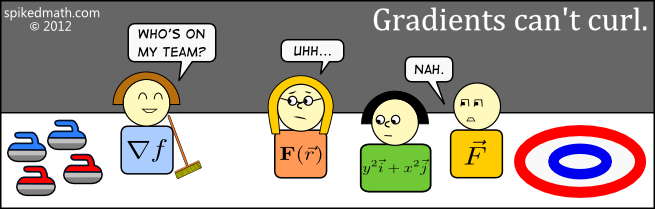
\includegraphics[width=10cm]{501-curling-with-gradients.png}
        {\tiny De \href{http://spikedmath.com/501.html}{Spiked math}, publié sous \href{http://creativecommons.org/licenses/by-nc-sa/2.5/ca/}{licence Creative Commons}.}
\end{center}

%+++++++++++++++++++++++++++++++++++++++++++++++++++++++++++++++++++++++++++++++++++++++++++++++++++++++++++++++++++++++++++
\section[Interprétation de la divergence]{Interprétation géométrique et physique de la divergence}
%+++++++++++++++++++++++++++++++++++++++++++++++++++++++++++++++++++++++++++++++++++++++++++++++++++++++++++++++++++++++++++

En physique, on dit qu'un champ de vecteurs à divergence nulle est \defe{incompressible}{incompressible!champ de vecteur}. Nous allons essayer de comprendre pourquoi. Lorsqu'un fluide incompressible se déplace, il faut qu'en chaque point il y autant de fluide qui rentre que de fluide qui sort. Nous allons voir sur quelques exemples que la divergence d'un champ de vecteurs est le «bilan de masse» d'un fluide qui se déplace selon le champ de vecteurs.

Si en un point la divergence est positive, cela signifie qu'il y a une perte de masse et si la divergence est négative, cela signifie qu'il y a une accumulation de masse.

Prenons par exemple un fluide qui se déplace selon le champ de vitesse montré à figure \ref{LabelFigBEHTooWsdrys}. % From file BEHTooWsdrys
\newcommand{\CaptionFigBEHTooWsdrys}{Le champ de vecteurs $F(x,y)=\frac{1}{ x }(1,0)$.}
\input{Fig_BEHTooWsdrys.pstricks}

Étant donné que la vitesse diminue lorsque $x$ avance, il y a une accumulation de fluide. Regardez en effet la quantité de fluide qui rentre dans le rectangle par rapport à la quantité de fluide qui en sort. Ce champ de vecteurs a pour équation :
\begin{equation}
    F(x,y)=\frac{1}{ x }\begin{pmatrix}
        1    \\ 
        0    
    \end{pmatrix}=\begin{pmatrix}
        1/x    \\ 
        0    
    \end{pmatrix}.
\end{equation}
Sa divergence vaut donc
\begin{equation}
    (\nabla\cdot F)(x,y)=\frac{ \partial F_x }{ \partial x }(x,y)+\underbrace{\frac{ \partial F_y }{ \partial y }(x,y)}_{=0}=-\frac{1}{ x^2 }.
\end{equation}
Cette divergence étant négative, il y a bien accumulation de fluide en tout point, et d'autant plus que $x$ est petit.

\begin{example}     \label{ExamDivFrot}

    Prenons le champ de vecteurs tournant
    \begin{equation}
        F(x,y)=\frac{1}{ \sqrt{x^2+y^2} }\begin{pmatrix}
            y    \\ 
            -x    
        \end{pmatrix}
    \end{equation}
    représenté à la figure \ref{LabelFigYQVHooYsGLHQ}. Cela est un vecteur qui est constamment perpendiculaire au rayon.


\newcommand{\CaptionFigYQVHooYsGLHQ}{Le champ de vecteurs $F(x,y)=(y,-x)$.}
\input{Fig_YQVHooYsGLHQ.pstricks}

    Un fluide dont la vitesse serait donné par ce champ de vecteur se contente de tourner. Intuitivement il ne devrait pas y avoir de divergence parce qu'il n'y a aucune accumulation de fluide. En effet,
    \begin{equation}
        \nabla\cdot F(x,y)=\frac{ -2xy }{ (x^2+y^2)^2 }+\frac{ 2xy }{ (x^2+y^2)^2 }=0.
    \end{equation}
\end{example}

\begin{example}
    Prenons le cas du champ de force de gravitation :
    \begin{equation}
        F(x,y,z)=\frac{1}{ (x^2+y^2+z^2)^{3/2} }\begin{pmatrix}
            x    \\ 
            y   \\
            z
        \end{pmatrix}.
    \end{equation}
    Nous pouvons rapidement remarquer que $\nabla\cdot F=0$. Est-ce que cela peut se comprendre sur le dessin de la figure \ref{LabelFigZGUDooEsqCWQ}. % From file ZGUDooEsqCWQ
\newcommand{\CaptionFigZGUDooEsqCWQ}{Le champ de vecteur de la gravité. Nous avons tracé, sur les deux cercles la même densité de vecteurs, c'est à dire le même nombre de vecteurs par unité de surface.}
\input{Fig_ZGUDooEsqCWQ.pstricks}

    Essayons de voir combien de fluide entre dans la zone bleue et combien en sort. D'abord, il est certain que les vecteurs qui sortent sont plus courts que ceux qui rentrent, ce qui voudrait dire qu'il y a plus de fluide qui rentre. Mais on voit également que le \emph{nombre} de vecteurs qui sortent est plus grand parce que la seconde sphère est plus grande et qu'il y a un vecteur en chaque point de la sphère.

    Intuitivement nous pouvons dire que la quantité qui rentre dans la sphère de rayon $r_1$ donnée par la taille des vecteurs entrants multiplié par la surface de la sphère, c'est à dire
    \begin{equation}        \label{EqQpinormeVecto}
        4\pi r_1^2\| F(x,y,z) \|,
    \end{equation}
    mais $\| F(x,y,z) \|=\frac{1}{ r_1^2 }$, donc la quantité de fluide entrant est $4\pi$. La quantité de fluide sortant sera la même.

    Cela explique deux choses
    \begin{enumerate}
        \item
            Pourquoi les forces de gravitation et électromagnétiques sont en $1/r^2$; c'est parce que nous vivons dans un monde avec trois dimensions d'espace. En étudiant très précisément le champ de gravitation, certains physiciens espèrent trouver des déviations expérimentales par rapport à la règle du \( 1/r^2\); cela \emph{pourrait} être un signe que l'espace contient des dimensions supplémentaires.
        \item
            Pourquoi il y a un $4\pi$ comme coefficient dans beaucoup d'équations en électromagnétisme; en particulier dans certaines anciennes unités de flux.
    \end{enumerate}
    
\end{example}

\begin{remark}
    Nous allons voir plus loin comment s'assurer que l'équation \eqref{EqQpinormeVecto} représente bien la «quantité de fluide» qui rentre dans la zone délimitée
\end{remark}


%+++++++++++++++++++++++++++++++++++++++++++++++++++++++++++++++++++++++++++++++++++++++++++++++++++++++++++++++++++++++++++
\section{Quelques formules de Leibnitz}
%+++++++++++++++++++++++++++++++++++++++++++++++++++++++++++++++++++++++++++++++++++++++++++++++++++++++++++++++++++++++++++

La divergence étant une combinaison de dérivées, il n'est pas tellement étonnant que la divergence de produits donne lieux à des formules en deux termes. Si $f$ est une fonction et si $F$ et $G$ sont des champs de vecteurs, nous avons (sans démonstrations) :
\begin{equation}        \label{EqLeinDivNablRot}
    \begin{aligned}[]
        \nabla\cdot(fF)&=f\nabla\cdot F+F\cdot\nabla f\\
        \nabla\cdot(F\times G)&=G\cdot\nabla\times F-F\cdot\nabla\times G.
    \end{aligned}
\end{equation}
Nous avons aussi, pour le rotationnel,
\begin{equation}        \label{EqLeinRotfFF}
    \nabla\times(fF)=f\nabla\times F+\nabla f\times F.
\end{equation}
% This is part of Mes notes de mathématique
% Copyright (c) 2011-2012
%   Laurent Claessens
% See the file fdl-1.3.txt for copying conditions.

%+++++++++++++++++++++++++++++++++++++++++++++++++++++++++++++++++++++++++++++++++++++++++++++++++++++++++++++++++++++++++++
\section{La différentielle revisitée}
%+++++++++++++++++++++++++++++++++++++++++++++++++++++++++++++++++++++++++++++++++++++++++++++++++++++++++++++++++++++++++++

%---------------------------------------------------------------------------------------------------------------------------
\subsection{Les formes différentielles de base}
%---------------------------------------------------------------------------------------------------------------------------

Si la fonction $f\colon \eR^n\to \eR$ est différentiable alors la différentielle en $a\in\eR^n$ est l'application
\begin{equation}        \label{EqFormDiffdfah}
    \begin{aligned}
        df_a\colon \eR^n&\to \eR \\
        u&\mapsto \frac{ \partial f }{ \partial x_1 }(a)u_1+\ldots+\frac{ \partial f }{ \partial x_n }(a)u_n.
    \end{aligned}
\end{equation}
Considérons en particulier la fonction qui à $x\in\eR^n$ fait correspondre $x_i\in\eR$. Par abus de notations,  nous la noterons $x_i$. Nous avons 
\begin{equation}
    \frac{ \partial x_i }{ \partial x_j }=\delta_{ij}.
\end{equation}
Par exemple $\partial_yx=0$ et $\partial_xx=1$. Toutes les dérivées partielles de $x_i$ s'annulent sauf la $i$ème qui vaut $1$. Par conséquent
\begin{equation}
    \begin{aligned}
        dx_i\colon \eR^n&\to \eR \\
        u&\mapsto u_i. 
    \end{aligned}
\end{equation}

\begin{remark}
    En toute rigueur nous devrions écrire $(dx_i)_a$. Mais étant donné que
    \begin{equation}
        (dx_i)_a(u)=(dx_i)_b(u)
    \end{equation}
    pour tout points $a$, $b$ et pour tout vecteurs $u$, nous nous permettons de simplifier la notation en ne précisant pas en quel point nous calculons la différentielle de $x_i$.
\end{remark}

Étant donné que $dx_i(u)=u_i$, nous pouvons récrire la formule \eqref{EqFormDiffdfah} en remplaçant $u_i$ par $dx_i(u)$ :
\begin{equation}
    df_a(u)=\frac{ \partial f }{ \partial x_1 }(a)dx_1(u)+\ldots+\frac{ \partial f }{ \partial x_n }(a)dx_n(u).
\end{equation}
En tant que application linéaire, $df_a$ est une combinaison linéaire des $dx_i$. En notations compacte :
\begin{equation}
    df_a=\sum_{i=1}^n\frac{ \partial f }{ \partial x_i }(a)dx_i.
\end{equation}

%---------------------------------------------------------------------------------------------------------------------------
                    \subsection{Différentielle comme élément de l'espace dual}
%---------------------------------------------------------------------------------------------------------------------------

Si nous considérons la base canonique $\{ e_i \}_{i=1,\ldots,n}$ de $\eR^n$. À partir d'elle, nous considérons la \defe{base duale}{base!duale}. En termes pratiques, nous définissons $dx_i$ comme la forme sur $\eR^n$ qui à un vecteur $u$ fait correspondre sa composante $i$ :
\begin{equation}
    dx_i\begin{pmatrix}
    u^1 \\ 
    \vdots  \\ 
    u^n 
\end{pmatrix}=u^i.
\end{equation}
En termes savants, $dx_i$ est le dual de $e_i$. Si tu ne l'as pas encore compris, Jean Doyen va te le faire comprendre !


Maintenant, dans la formule \eqref{EqDiffPartRap}, nous pouvons remplacer $u^i$ par $dx_i(u)$, et écrire
\begin{equation}
    df_a(u)=\sum_i\frac{ \partial f }{ \partial x_i }(a)u^i=\sum_i\frac{ \partial f }{ \partial x_i }(a)dx_i(u).
\end{equation}
Ce qui arrive tout à droite est explicitement vu comme une forme sur $\eR$, dont les composantes dans la base duale sont les dérivées partielles de $f$ au point $a$, agissant sur $u$. En faisant un pas en arrière, nous omettons le $u$, et nous écrivons
\begin{equation}
    df_a=\sum_{i=1}^n\frac{ \partial f }{ \partial x_i }(a)dx^i
\end{equation}

Cette notation $dx_i$ pour la forme duale de $e_i$ est en réalité parfaitement logique parce que $dx^i$ est la différentielle de la projection
\begin{equation}
    \begin{aligned}
        x^i\colon \eR^n&\to \eR \\
        (x^1,\ldots,x^n)&\mapsto x^i. 
    \end{aligned}
\end{equation}
Je te laisse un peu méditer sur cette différentielle de la projection. L'important est que tu aies compris cela d'ici la fin de ta deuxième année.

%---------------------------------------------------------------------------------------------------------------------------
\subsection{Différentielles de fonctions composées}
%---------------------------------------------------------------------------------------------------------------------------

Cette façon de voir la différentielle nous permet de jeter un nouveau regard sur la formule de différentiation des fonctions composées. Soient
\begin{equation}
    \begin{aligned}[]
        f\colon \eR^p&\to \eR^n\\
        g\colon \eR^n&\to \eR,
    \end{aligned}
\end{equation}
et $h\colon \eR^p\to \eR$ définie par 
\begin{equation}
    h(u)=h\big( f(u) \big)=(g\circ f)(u).
\end{equation}
Nous allons noter $x$ les coordonnées de $\eR^p$, $a$ un point de $\eR^p$ et $u$, un vecteur de $\eR^p$ accroché au point $a$. Pour $\eR^n$, les notations seront que les coordonnées sont $y$, $b$ est un point de $\eR^n$ et $v$ est un vecteur «accroché» au point $b$.

Nous avons
\begin{equation}
    dg_b(v)=\sum_{i=1}^n\frac{ \partial g }{ \partial y_i }(b)dy_i(v).
\end{equation}
Ici $dy_i(v)$ signifie la $i$ème composante de $v$. C'est simplement $v_i$. Cette formule étant valable pour tout point $b\in\eR^n$ et pour tout vecteur $v$, nous pouvons l'écrire en particulier pour
\begin{subequations}
    \begin{numcases}{}
        b=f(a)\\
        v=df_a(u).
    \end{numcases}
\end{subequations}
Cela donne
\begin{equation}        \label{Eqdgfadfau}
    dg_{f(a)}\big( df_a(u) \big)=\sum_{i=1}^n\frac{ \partial g }{ \partial y_i }\big( f(a) \big)dy_i\big( df_a(u) \big).
\end{equation}
Mais 
\begin{equation}
    df_a(u)=\sum_{j=1}^p\frac{ \partial f }{ \partial x_j }(a)dx_j(u),
\end{equation}
donc la $i$ème composante de ce vecteur est
\begin{equation}
     \big( df_a(u)\big)_i=\sum_{j=1}^p\frac{ \partial f_i }{ \partial x_j }(a)dx_j(u).
\end{equation}
En remplaçant $dy_i\big( df_a(u) \big)$ par cela dans l'expression \eqref{Eqdgfadfau}, nous trouvons
\begin{equation}
    dg_{f(a)}\big( df_a(u) \big)=\sum_{i=1}^n\frac{ \partial g }{ \partial y_i }\big( f(a) \big)\sum_{j=1}^p\frac{ \partial f_i }{ \partial x_j }(a)dx_j(u).
\end{equation}
Nous pouvons vérifier que cela est la différentielle de $g\circ f$ au point $a$ appliquée au vecteur $u$. En effet
\begin{equation}
    d(g\circ f)_a(u)=\sum_{j=1}^p\frac{ \partial (g\circ f) }{ \partial x_j }(a)dx_j(u),
\end{equation}
tandis que, par la dérivation de fonctions composées, 
\begin{equation}        \label{EqDerCompofg}
    \frac{ \partial (g\circ f) }{ \partial x_j }(a)=\sum_{i=1}^n\frac{ \partial g }{ \partial y_i }\big( f(a) \big)\frac{ \partial f_i }{ \partial x_j }(a).
\end{equation}
Au final, ce que nous avons prouvé est que
\begin{equation}
    d(g\circ f)_a(u)=dg_{f(a)}\big( df_a(u) \big).
\end{equation}

%---------------------------------------------------------------------------------------------------------------------------
\subsection{Exemple de composée : les coordonnées polaires}
%---------------------------------------------------------------------------------------------------------------------------

Le changement de coordonnées pour les polaires est la fonction
\begin{equation}
    f\begin{pmatrix}
        r    \\ 
        \theta    
    \end{pmatrix}=\begin{pmatrix}
        x    \\ 
        y    
    \end{pmatrix}=\begin{pmatrix}
        r\cos\theta    \\ 
        r\sin\theta    
    \end{pmatrix}.
\end{equation}
Considérons une fonction $g$ sur $\eR^2$, et définissons la fonction $\tilde g$ par
\begin{equation}
    \tilde g(r,\theta)=g(r\cos\theta,r\sin\theta).
\end{equation}
La formule \eqref{EqDerCompofg} permet de trouver les dérivées partielles de $g$ par rapport à $r$ et $\theta$ en termes de celles par rapport à $x$ et $y$ de $g$.

Pour faire le lien avec les notations du point précédent, nous avons
\begin{equation}
    \begin{aligned}[]
        f_1(r,\theta)&=r\cos(\theta)\\
        f_2(r,\theta)&=r\sin(\theta)\\
        (x_1,x_2)&\to(r,\theta)\\
        (y_1,y_2)&\to(x,y).
    \end{aligned}
\end{equation}
Nous avons donc 
\begin{equation}
    \begin{aligned}[]
        \frac{ \partial \tilde g }{ \partial r }(r,\theta)&=\sum_{i=1}^2\frac{ \partial g }{ \partial x_i }\big( f(r,\theta) \big)\frac{ \partial f_i }{ \partial r }(r,\theta)\\
        &=\frac{ \partial g }{ \partial x }(r\cos\theta,r\sin\theta)\frac{ \partial \big( r\cos\theta \big) }{ \partial r }(r,\theta)\\
        &\quad+\frac{ \partial g }{ \partial y }(r\cos\theta,r\sin\theta)\frac{ \partial \big( r\sin\theta\big) }{ \partial r }(r,\theta)\\
        &=\cos\theta\frac{ \partial g }{ \partial x }(r\cos\theta,r\sin\theta)+\sin\theta\frac{ \partial g }{ \partial y }(r\cos\theta,r\sin\theta).
    \end{aligned}
\end{equation}

Prenons par exemple $g(x,y)=\frac{1}{ x^2+y^2 }$. Étant donné que
\begin{equation}
    \frac{ \partial g }{ \partial x }=\frac{ -2x }{ (x^2+y^2)^2 },
\end{equation}
nous avons
\begin{equation}
    \frac{ \partial g }{ \partial x }(r\cos\theta,r\sin\theta)=\frac{ -2\cos\theta }{ r^3 }.
\end{equation}
En utilisant la formule,
\begin{equation}
    \frac{ \partial \tilde g }{ \partial r }(r,\theta)=\cos(\theta)\left( \frac{ -2\cos\theta }{ r^3 } \right)+\sin(\theta)\left( \frac{ -2\sin\theta }{ r^3 } \right)=-\frac{ 2 }{ r^3 }.
\end{equation}
Nous pouvons vérifier directement que cela est correct. En effet
\begin{equation}
    \tilde g(r,\theta)=g(r\cos\theta,r\sin\theta)=\frac{1}{ r^2 },
\end{equation}
dont la dérivée par rapport à $r$ vaut $-2/r^3$.

En ce qui concerne la dérivée par rapport à $\theta$, nous avons
\begin{equation}
    \begin{aligned}[]
    \frac{ \partial \tilde g }{ \partial \theta }&=\frac{ \partial g }{ \partial x }(r\cos\theta,r\sin\theta)\frac{ \partial \big( r\cos(\theta) \big) }{ \partial \theta }+\frac{ \partial g }{ \partial y }(r\cos\theta,r\sin\theta)\frac{ \partial \big( r\sin(\theta) \big) }{ \partial \theta }\\
    &=\left( \frac{ -2\cos\theta }{ r^3 } \right)(-r\sin\theta)+\left( \frac{ -2\sin\theta }{ r^3 } \right)(r\cos\theta)\\
    &=0.
    \end{aligned}
\end{equation}

En résumé et avec quelques abus de notations :
\begin{equation}
    \begin{aligned}[]
        \frac{ \partial \tilde g }{ \partial r }&=\cos(\theta)\frac{ \partial g }{ \partial x }+\sin(\theta)\frac{ \partial g }{ \partial y }\\
        \frac{ \partial \tilde g }{ \partial \theta }&=-r\sin(\theta)\frac{ \partial g }{ \partial x }+r\cos(\theta)\frac{ \partial g }{ \partial y }\\
    \end{aligned}
\end{equation}
